% !TEX root = ./Basilisk-ephemDifference-2019-03-27.tex


\begin{figure}[h]
	\centerline{
		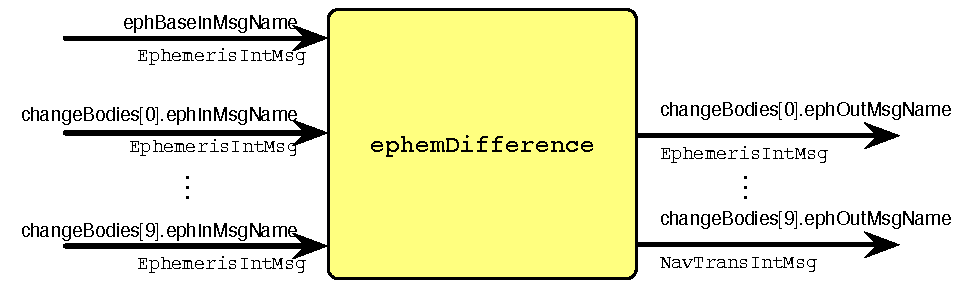
\includegraphics{Figures/moduleImg}
	}
	\caption{Illustration of the module input and output messages.}
	\label{fig:moduleImg}
\end{figure}


\section{Model Description}
The purpose of this module is to rebase ephemeris position and velocity vectors relative to another celestial object.  All the input messages are assumed to have the vectors taken with respect to the same coordinate frame.

Let $\bm r_{P_{i}/N}$ be the position vector of the $i^{\text{th}}$ ephemeris, while $\bm r_{B/N}$ is the position vector of the bases ephemeris message.  The velocity vectors $\bm v_{P_{i}/N}$ and $\bm v_{B/N}$ are defined similarly.  Taking all vectors components with respect to a command inertial frame $\cal N$, the output is computed using
\begin{align}
	\leftexp{N}{\bm r}_{P_{i}/B} &= \leftexp{N}{\bm r}_{P_{i}/N} - \leftexp{N}{\bm r}_{B/N}
	\\
	\leftexp{N}{\bm v}_{P_{i}/B} &= \leftexp{N}{\bm v}_{P_{i}/N} - \leftexp{N}{\bm v}_{B/N}
\end{align}

The time tag of the output message is copied from the corresponding input message, not the base ephemeris message.

The number of input messages to consider is determined by searching the {\tt ephInMsgName} and {\tt ephOutMsgName} names and finding the first zero string where either name was not set.  

